\subsection{Exemples de stratégies}
\url{http://view.eecs.berkeley.edu/wiki/Dwarf_Mine}

Le choix des opérateurs dans Taggre se fait à l'appréciation du programmeur.
%
La collection des {\em 13 nains de Berkeley} est une méthode de classification des problèmes suivant leurs motifs de calculs et de communication.
%
Il est intéressant de voir si Taggre peut répondre aux 13 problèmes et si c'est le cas quelle serait la stratégie d'agrégation à utiliser.



\subsubsection{}
Dans le cas d'un graphe étant plus large que haut, nous pouvons utiliser l'opérateur F.
%
Celui-ci nous permettra de diminuer le nombre de tâche en diminuant le parallélisme.
%
Ce genre de graphe peuvent être utilisés dans les méthodes spectrales.


%   (-_-)   %
\begin{figure}[t!]
  \centering
  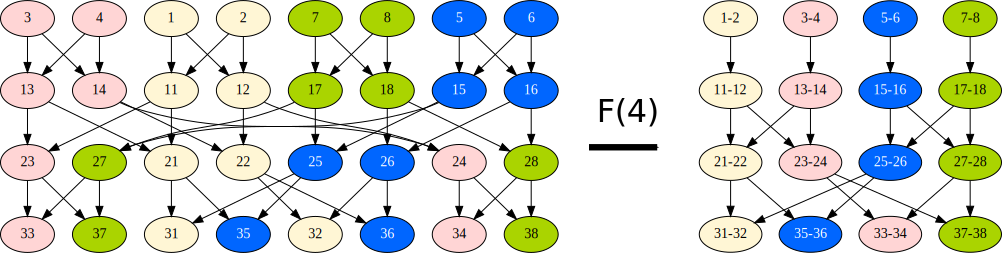
\includegraphics[width=\textwidth]{dwarf_spec}
  \caption{Exemple d'agrégation sur un graphe de méthode spectrale.}
  \label{fig:dwarf_spec}
\end{figure}



\subsubsection{Les arbres}
